%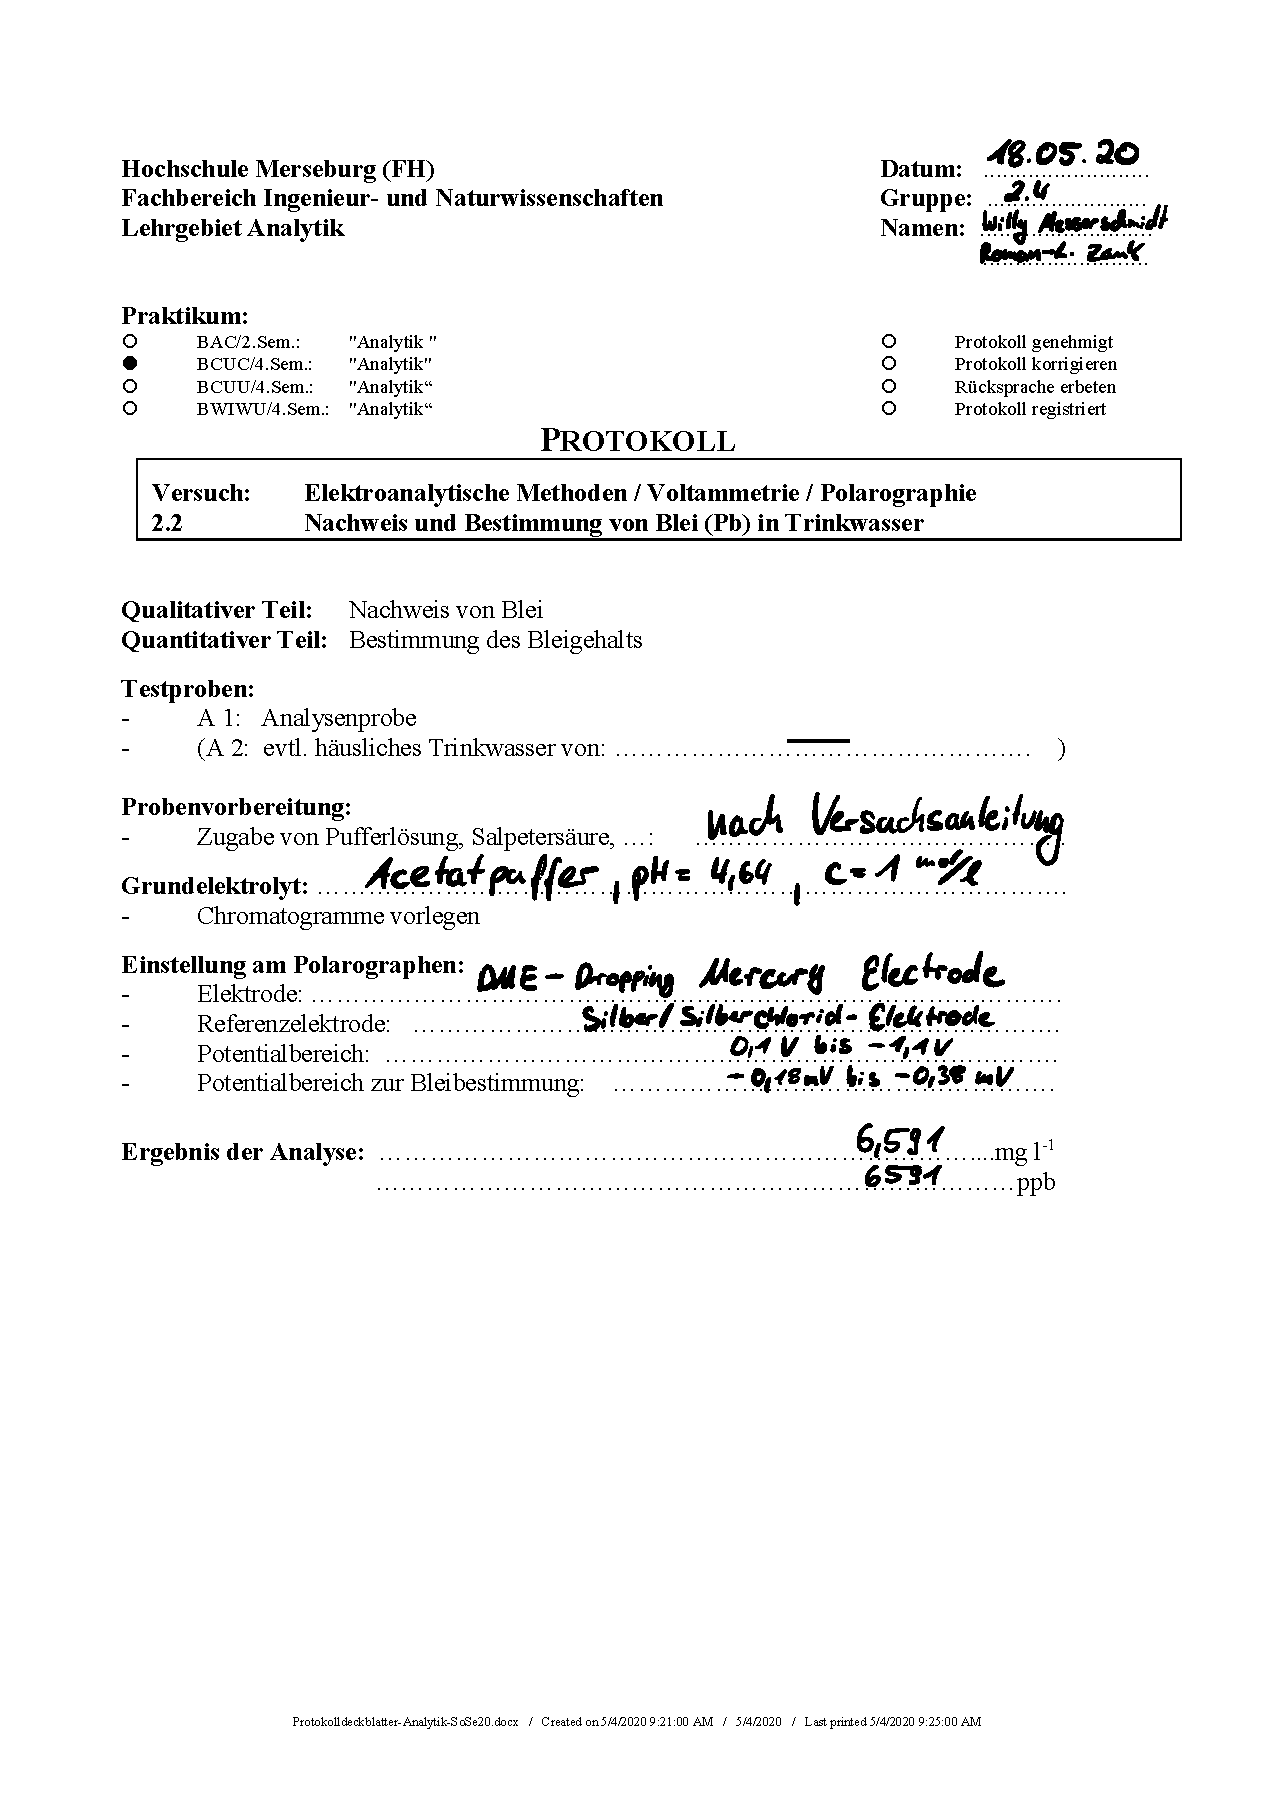
\includepdf[]{Deckblatt}
\pagebreak
\section{Einleitung}
\label{sec:einleitung}
Im folgenden Protokoll werden generierte Messdaten zum Versuch \textit{WÜK} ausgewertet. Ziel ist es mit Hilfe der erklärenden Videos zum Praktikum und Mittels der gegebenen Messdaten den Wärmeübergangskoeffizient $\alpha_L$ für turbulente Luftströmungen zu bestimmen. Dafür werden  drei verschiedene Rohre unter unterschiedlichen Volumenströmen der Luft untersucht. Die Wärmeübertragung mit Wasser erfolgt  in diesem Versuch mittels Gleichstrom.
Darüber hinaus sind, mittels Nusseltzahl $Nu$ und der Nusseltparameter $a$ und $b$, Bewertungen zur Wärmeübertragung der verschiedenen Rohre und Volumenströme abzugeben.





